\documentclass[runningheads]{llncs}
\usepackage[T1]{fontenc}
\usepackage{graphicx}
\usepackage{subcaption}
\usepackage{multirow}
\usepackage[normalem]{ulem}
\useunder{\uline}{\ul}{}
\usepackage{amsmath}

\begin{document}
\title{Deep Learning Based Methods for Phage Contig Prediction}
\author{
Son Vu Quang\inst{1} \and
Diep Thi Hoang\inst{1}
% Third Author\inst{3}\orcidID{2222--3333-4444-5555}
}

\institute{
University of Engineering and Technology, Vietnam National University, Hanoi, Vietnam
}

\maketitle              % typeset the header of the contribution

\begin{abstract}
Bacteriophages are classified into two distinct lifestyle categories—virulent and temperate—based on their replicative strategies. Accurate lifestyle prediction is essential for elucidating phage-host interactions within microbial communities and for developing effective phage therapy applications. While computational methods have emerged as viable alternatives to time-consuming laboratory approaches, existing tools demonstrate suboptimal performance on short DNA fragments commonly encountered in metagenomic assemblies. This study presents PhaBERT-CNN, a deep learning framework leveraging the DNABERT-2\cite{zhou2023dnabert} pre-trained foundation model for phage lifestyle classification from metagenomic contigs. We conducted comprehensive performance evaluations across four contig length ranges (100-400 bp, 400-800 bp, 800-1200 bp, and 1200-1800 bp) and compared our approach against state-of-the-art methods, including PhaTYP\cite{shang2023phatyp}, DeePhage\cite{wu2021deephage}, and ProkBERT\cite{ligeti2024prokbert}. PhaBERT-CNN demonstrates superior performance on short to medium-length contigs (Groups A-C: 100-1200 bp), outperforming all competing methods with accuracy improvements of 0.91-2.67\% over PhaTYP, 2.17-3.24\% over DeePhage, and 0.91-5.98\% over ProkBERT. Specifically, the model achieves sensitivity values of 82.00\%-91.12\%, specificity of 80.15\%-85.93\%, and overall accuracy of 81.59\%-90.01\% across these challenging length ranges. For the longest contig group D (1200-1800 bp), where PhaTYP demonstrates its strongest performance, PhaBERT-CNN achieves competitive results with 88.47\% sensitivity, 90.95\% specificity, and 90.69\% accuracy, trailing PhaTYP by only 0.34\% in accuracy while maintaining superior performance over DeePhage (2.03\% improvement) and ProkBERT (5.96\% improvement). This balanced performance profile positions PhaBERT-CNN as a robust solution for metagenomic phage lifestyle classification across the complete spectrum of contig lengths typically encountered in assembly workflows.

\keywords{Bacteriophage lifestyle prediction, DNABERT-2, virulent phage, temperate phage, metagenomics, deep learning}
\end{abstract}
%
%
%
\section{Introduction}
Bacteriophages (phages) are viruses that specifically infect bacteria and play critical roles as regulators of microbial ecology and as promising antimicrobial therapeutic agents. Phages are classified into two major lifestyle categories based on their replicative strategies\cite{wu2021deephage}. Virulent phages (also known as strictly lytic phages) exclusively undergo lytic infection, rapidly hijacking the host cellular machinery to produce progeny virions and causing host cell lysis\cite{mcnair2012phacts}. In contrast, temperate phages (also known as lysogenic phages) can establish lysogeny by integrating their genetic material into the host chromosome as a prophage, where they remain dormant and replicate along with the host genome until environmental stressors trigger the transition to lytic replication\cite{mcnair2012phacts}.

Accurate classification of phages into virulent or temperate categories is essential for both microbiome research and therapeutic applications\cite{shang2023phatyp}. Such classification elucidates complex phage-host interactions and clarifies the ecological roles of phages within microbial communities\cite{shang2023phatyp}. Moreover, identifying virulent phages is a prerequisite for developing effective phage therapy strategies to combat pathogenic bacteria, offering promising alternatives to conventional antibiotics\cite{azimi2019phage}. Traditional experimental methods for phage lifestyle determination rely on laboratory cultivation and phenotypic observation, approaches that are time-consuming, labor-intensive, and inapplicable to the vast majority of unculturable phages present in environmental samples\cite{shang2023phatyp}. These limitations have driven the development of computational methods for rapid, scalable phage lifestyle prediction directly from sequence data. In metagenomic analyses, phage genomes are typically recovered as contigs—contiguous sequences assembled from overlapping short reads\cite{setubal2021metagenome,ghurye2016metagenomic}. These contigs often exhibit substantial length variation and fragmentation due to uneven sequencing coverage, technical artifacts, and repetitive genomic regions, making the development of tools that can accurately classify incomplete sequences a critical computational challenge.

Computational approaches for phage lifestyle prediction face significant challenges due to four primary factors: data limitations, absence of characteristic marker genes, short DNA fragment lengths, and sequence similarity issues. First, existing phage genome databases remain severely limited due to the vast diversity of phages in nature, the majority of which have not yet been isolated and characterized\cite{hayes2017metagenomic}. Second, bacteriophages lack universal marker genes analogous to the 16S ribosomal RNA gene found in bacteria, rendering marker gene-based classification approaches infeasible\cite{mokili2012metagenomics}. Furthermore, metagenomic data typically contain numerous short DNA fragments comprising only partial genes or incomplete gene sequences, complicating functional gene-based classification strategies\cite{jiang2017ensvmb}. Finally, bacteriophages may share genetic sequences with their bacterial hosts through horizontal gene transfer, potentially leading to misclassification during taxonomic assignment\cite{rozov2017recycler}.

Given these challenges, the phage lifestyle prediction problem can be formally stated as follows: given a set of contigs $\mathcal{S} = \{S_1, S_2, \ldots, S_n\}$ obtained from metagenomic sequencing and assembly, where each contig $S_i$ has length $L_i$ base pairs, the task is to predict the lifestyle of the phage as either virulent (lytic) or temperate (lysogenic).

In this paper, we propose PhaBERT-CNN, a novel hybrid deep learning framework that integrates the pre-trained DNABERT-2\cite{zhou2023dnabert} model with multi-scale convolutional neural networks for accurate phage lifestyle prediction. Our approach leverages transfer learning from DNABERT-2\cite{zhou2023dnabert} model to capture contextual evolutionary patterns in phage DNA sequences, while utilizing parallel CNN branches with multiple receptive fields to extract local sequence features from the learned embeddings and attention-based pooling mechanism to aggregate global sequence-level information from the transformer representations.

The remainder of this paper is organized as follows. Section \ref{related_works} provides a comprehensive review of related work in phage lifestyle prediction. Section \ref{method} describes our proposed PhaBERT-CNN methodology. Section \ref{results} presents the experimental setup, including dataset construction, evaluation metrics, and comparative analysis with state-of-the-art methods. Finally, Section \ref{discussion} analyzes the experimental results.

\section{Related work} \label{related_works}
Recognizing the critical importance of this classification challenge, numerous computational approaches have been developed for bacteriophage identification. Early methods utilized traditional machine learning algorithms, with prominent tools including PHACTS\cite{mcnair2012phacts}, PhageAI\cite{tynecki2020phageai}, and BACPHLIP\cite{hockenberry2021bacphlip}. The advancement of parallel computing technologies has enabled the development and publication of sophisticated deep learning-based models, such as DeePhage\cite{wu2021deephage}, PhaTYP\cite{shang2023phatyp}, and DeepPL\cite{zhang2024deeppl}. These technological advances have led to progressive improvements in classification performance, making computational bacteriophage classification increasingly viable for real-world applications.

Methods based on machine learning, such as PHACTS\cite{mcnair2012phacts}, PhageAI\cite{tynecki2020phageai}, and BACPHLIP\cite{hockenberry2021bacphlip}, utilize complete genomic datasets. With these datasets, these methods have achieved remarkably high performance, with most attaining classification accuracies exceeding 90\%. PHACTS employs a two-step genetic data encoding process: (1) creating a standard protein set, and (2) generating similarity vectors for proteins in the bacteriophage genomic dataset using the FASTA tool, then concatenating these vectors to produce the final encoding vector. PHACTS\cite{mcnair2012phacts} utilizes the Random Forest algorithm for training and classification. PhageAI\cite{tynecki2020phageai} has successfully applied natural language processing techniques to genetic data, achieving excellent results. The method uses k-mers to convert genetic sequences into text format, followed by Word2Vec for feature encoding. Additionally, PhageAI\cite{tynecki2020phageai} employs Recursive Feature Elimination with Cross-Validation (RFECV) to remove redundant features, retaining only those with a significant impact on classification performance. The authors experimented with multiple models, with the Support Vector Machine (SVM) algorithm yielding optimal performance. BACPHLIP\cite{hockenberry2021bacphlip} focuses on exploiting conserved protein regions for data encoding. Conserved protein regions represent functional domains inherited across multiple generations. The authors encode data through a two-step process: (1) identifying conserved protein regions, and (2) creating binary feature vectors representing the presence of these conserved regions. The method employs the Random Forest algorithm and demonstrates competitive performance. However, the limited availability of data on conserved protein regions poses challenges for practical application.

As noted above, the machine learning-based tools discussed are designed to handle problems under ideal conditions where inputs consist of complete genomic datasets. When applied to fragmented sequences (contigs), these methods demonstrate substantially degraded performance compared to deep learning-based approaches such as DeePhage\cite{wu2021deephage}, PhaTYP\cite{shang2023phatyp}, and DeepPL\cite{zhang2024deeppl}. According to results published in DeePhage\cite{wu2021deephage}, PHACTS\cite{mcnair2012phacts} exhibits approximately 30\% lower classification accuracy on bacteriophage contig datasets compared to complete genomes. DeePhage\cite{wu2021deephage} represents an early deep learning approach that employs Convolutional Neural Networks (CNNs) for bacteriophage classification. However, DeePhage suffers from several limitations that constrain its performance on short contigs. First, the CNN architecture has limited receptive field capacity, restricting its ability to capture long-range dependencies and global genomic patterns essential for accurate classification of fragmented sequences\cite{wu2021deephage}. Second, as a model trained from scratch without leveraging pre-trained representations, DeePhage lacks the prior biological knowledge that could enhance its ability to generalize across diverse genomic contexts, particularly when analyzing incomplete sequences with limited contextual information.

PhaTYP\cite{shang2023phatyp} is a tool based on BERT\cite{devlin2019bert}, a transformer model originally developed for natural language processing tasks. The authors adapted and fine-tuned BERT to classify genetic data for bacteriophage identification. While PhaTYP demonstrates improved performance over traditional methods, it exhibits critical dependencies that limit its applicability to short contigs. Specifically, PhaTYP relies on Prodigal\cite{hyatt2010prodigal} for protein-coding gene prediction and constructs a protein-based token vocabulary for sequence encoding. This protein-centric approach becomes problematic when applied to short contigs. Gene prediction tools like Prodigal show substantially decreased performance on fragments shorter than 200 bp\cite{trimble2012short}, and the fragmented nature of metagenomic assemblies may not contain complete gene sequences necessary for accurate protein identification\cite{shang2023phatyp}. This dependency on reliable gene prediction limits PhaTYP's applicability to highly fragmented sequences. Consequently, PhaTYP's performance degrades substantially when processing contigs below certain length thresholds, where gene prediction becomes unreliable.

DeepPL\cite{zhang2024deeppl} employs a similar transformer-based approach to PhaTYP but utilizes DNABERT\cite{ji2021dnabert}, a BERT-based model pre-trained specifically on genomic DNA sequences rather than protein sequences. While DNABERT provides advantages through domain-specific pre-training on genomic data, it is constrained by fundamental limitations in its tokenization strategy\cite{zhou2023dnabert}. DNABERT employs overlapping k-mer tokenization (typically k=6), which introduces significant information leakage during masked language modeling, as adjacent tokens share k-1 nucleotides. Furthermore, overlapping k-mer tokenization suffers from poor computational efficiency\cite{zhou2023dnabert}. For an input sequence of length L, the tokenized representation consists of L-k+1 tokens, each of length k, resulting in a sequence with considerable redundancy and length nearly equivalent to the original sequence. Similarly, ProkBERT\cite{ligeti2024prokbert} employs overlapping k-mer tokenization through its Local Context-Aware (LCA) method and consequently shares these same limitations of information leakage and reduced sample efficiency\cite{zhou2023dnabert,ligeti2024prokbert}.

% These limitations underscore the need for models that can efficiently process variable-length genomic sequences without information leakage or dependency on external gene prediction tools. DNABERT-2\cite{zhou2023dnabert} addresses these challenges through Byte Pair Encoding tokenization, which eliminates information leakage while maintaining efficiency, and Attention with Linear Biases\cite{press2021train}, which enables flexible sequence length handling. Combined with multi-species pre-training, these innovations make DNABERT-2 particularly suitable for analyzing fragmented metagenomic sequences.

% Motivated by these advantages, we propose PhaBERT-CNN, a hybrid approach that leverages DNABERT-2 embeddings combined with convolutional neural networks (CNNs) as classifiers for bacteriophage lifestyle prediction. This method operates directly on raw DNA sequences, eliminating the dependency on gene prediction tools and enabling accurate classification even on short contigs, as presented in Section \ref{method}.

\section{Material and Methods} \label{method}
This section describes our PhaBERT-CNN methodology for phage lifestyle classification from metagenomic contigs. We first present the dataset construction process, including data sources and contig generation strategies that simulate real-world metagenomic scenarios. We then introduce the DNABERT-2\cite{zhou2023dnabert} foundation model, highlighting its key innovations in tokenization, architecture, and multi-species pre-training that enable effective processing of fragmented genomic sequences. Finally, we detail the PhaBERT-CNN architecture, which combines DNABERT-2's contextual embeddings with multi-scale convolutional layers to extract discriminative features for binary classification of virulent and temperate phages.

\subsection{Data construction}\label{data_construction}
To construct our dataset, we integrated data from two recent studies: DeePhage\cite{wu2021deephage} and DeepPL\cite{zhang2024deeppl}. Specifically, our dataset comprises the original DeePhage\cite{wu2021deephage} dataset supplemented with newly annotated sequences labeled as presented in DeepPL\cite{zhang2024deeppl}. The combined dataset includes 2,241 complete phage genomes (707 temperate, 1,534 virulent), with labels 0 and 1, respectively. We further used stratified $k$-fold cross-validation with $k=5$ and split each fold into a training set and a validation set with a ratio of 8:2.

To simulate real-world metagenomic scenarios, we generated contigs of varying lengths from the complete genomes using a sliding window approach. For each window, the length was randomly sampled from a normal distribution, and consecutive windows overlapped by a specified percentage. Following the methodology described in DeePhage\cite{wu2021deephage}, we initially created contigs in four length categories: A (100-400 bp), B (400-800 bp), C (800-1200 bp), and D (1200-1800 bp). The overlapping percentage varied across length categories: shorter contig groups employed lower overlap percentages to prevent excessive data generation, while longer contig groups utilized higher overlap rates. Following contig generation, we performed data augmentation by generating reverse complement sequences for all contigs. Finally, we applied random undersampling on the training set to address the class imbalance (virulent to temperate ratio of approximately 2:1). Although this approach may result in some information loss, it represents a necessary trade-off given our available computational resources.

\subsection{DNABERT-2 model}
To leverage pre-trained knowledge from diverse genomic sequences, we employed DNABERT-2\cite{zhou2023dnabert}, a state-of-the-art genome foundation model that addresses critical limitations in traditional k-mer-based tokenization approaches. Unlike its predecessor DNABERT\cite{ji2021dnabert}, which utilized overlapping k-mer tokenization on human genome sequences, DNABERT-2 introduces several methodological innovations that enhance both computational efficiency and model performance.

\textbf{Tokenization Strategy}. The tokenization procedure in DNABERT-2 leverages Byte Pair Encoding (BPE) \cite{sennrich2015neural} within the SentencePiece framework \cite{kudo2018sentencepiece} to segment DNA sequences. This approach constructs a vocabulary of variable-length subword tokens by iteratively merging the most frequently co-occurring nucleotide segments in the training corpus. Compared to k-mer tokenization, BPE offers three key advantages: (1) elimination of information leakage inherent in overlapping k-mer approaches, where adjacent tokens share k-1 nucleotides and inadvertently reveal information about masked positions; (2) approximately 5-fold reduction in sequence length, significantly improving computational efficiency; and (3) natural transformation of the masked language modeling objective into a span prediction task, where masked tokens of variable length require the model to predict both the number of nucleotides and their identities, which has been demonstrated to enhance learning effectiveness \cite{raffel2020exploring}.
\begin{figure}[h]
    \centering
    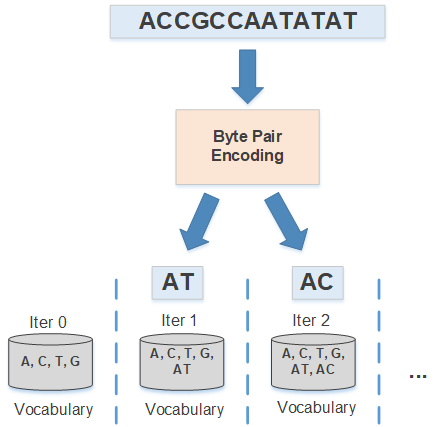
\includegraphics[width=0.5\linewidth]{imgs/bpe.png}
    \caption{BPE vocabulary construction example.}
    \label{fig:bpe}
\end{figure}

\textbf{Model Architecture}. The model architecture incorporates several technical enhancements to overcome the limitations of previous genome foundation models. DNABERT-2 replaces learned positional embeddings with Attention with Linear Biases (ALiBi) \cite{press2021train}, enabling the model to process arbitrarily long sequences without hard input length constraints. Additionally, Flash Attention\cite{dao2022flashattention} is integrated to reduce memory consumption and accelerate training, making the model 3× more efficient than DNABERT while using only one-third of the FLOPs despite having 30\% more parameters.

\textbf{Pre-training Corpus}. DNABERT-2 was pre-trained on a multi-species genome corpus encompassing diverse organisms, addressing the single-species limitation of DNABERT. This multi-species training strategy enhances the ability of model to capture conserved genomic patterns across evolutionary lineages while maintaining strong performance on species-specific tasks. The pre-training employed masked language modeling with an average sequence length of approximately 700 base pairs.

\textbf{Performance and Efficiency}. On the Genome Understanding Evaluation (GUE) benchmark—a comprehensive dataset comprising 36 tasks across 9 genomic analysis categories with sequences ranging from 70 to 10,000 bp, DNABERT-2 achieves performance comparable to the 2.5B-parameter Nucleotide Transformer\cite{dalla2025nucleotide} while being 21× smaller and requiring approximately 92× less GPU time during pre-training. The model demonstrates consistent performance across varying sequence lengths, effectively handling inputs 10× shorter or 15× longer than those encountered during pre-training. For phage-related genomic analysis, we utilized the pre-trained DNABERT-2 model, fine-tuning it on our specific downstream tasks following standard transfer learning protocols.

\subsection{PhaBERT-CNN Architecture and Training Strategy}

\begin{figure}[h]
    \centering
    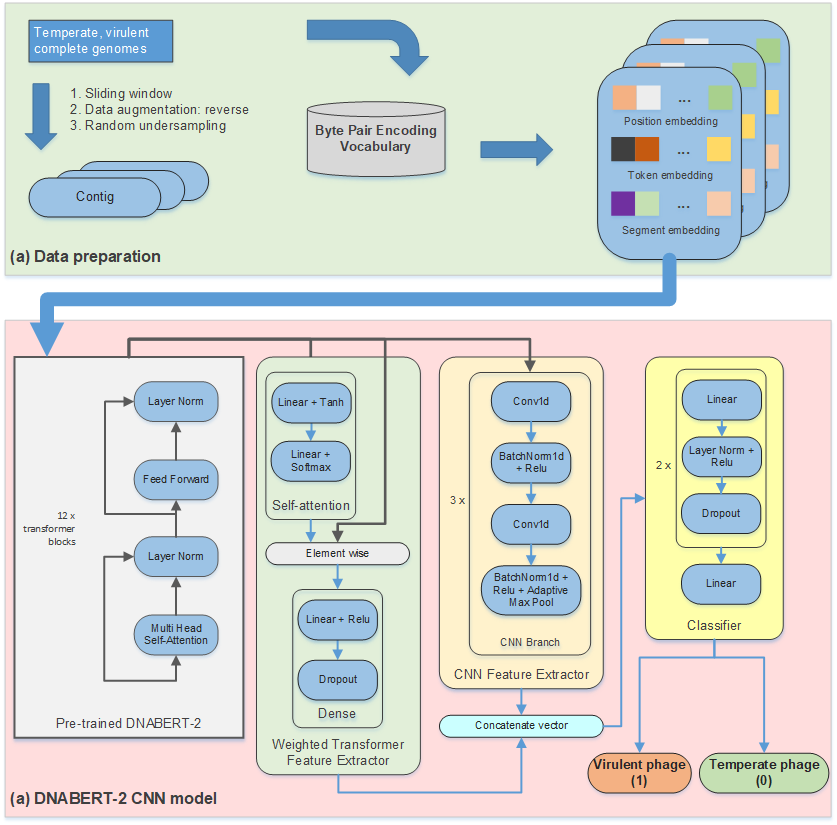
\includegraphics[width=1\linewidth]{imgs/my_pipeline.png}
    \caption{An overview of DNABERT-2-based pipeline for predicting phage lifestyle.}
    \label{fig:phabert-cnn}
\end{figure}

\subsubsection{Model Architecture.}

The PhaBERT-CNN architecture integrates pre-trained DNABERT-2 representations with task-specific feature extraction layers to enable effective phage lifestyle classification from metagenomic contigs. The model comprises three principal components: (1) the pre-trained DNABERT-2 backbone serving as a feature extractor, (2) dual parallel feature extraction branches processing the learned representations, and (3) a final classification head combining multi-scale features.

The pre-trained DNABERT-2\cite{zhou2023dnabert} model produces 768-dimensional contextualized embeddings for each tokenized sequence position, which serve as input to our downstream feature extraction architecture. We incorporate two parallel branches that operate on these learned representations to capture complementary aspects of phage genomic signatures:

\textbf{(1) Multi-scale CNN feature extractor}: Inspired by the Inception architecture \cite{szegedy2015going}, this branch employs three parallel convolutional pathways with varying kernel sizes (3, 5, and 7) to capture local sequence patterns at multiple spatial scales. Motivated by successful applications of CNNs on pre-trained embeddings in natural language processing \cite{kim2014convolutional,johnson2017deep}, we employ convolutional layers to learn task-specific feature transformations from the generic DNABERT-2 representations. The multi-scale architecture enables detection of discriminative patterns at multiple levels of abstraction—from fine-grained local motifs (kernel size 3) to broader functional domains (kernel sizes 5-7)—allowing hierarchical feature learning suitable for phage lifestyle classification \cite{johnson2017deep,szegedy2015going}. Each convolutional branch processes the 768-dimensional DNABERT-2 embeddings through two stacked Conv1d layers with progressive channel reduction (768 $\rightarrow$ 256 $\rightarrow$ 128), incorporating BatchNorm1d and ReLU activation after each convolution. Specifically, the first convolutional layer reduces the embedding dimension from 768 to 256 channels, while the second layer further compresses the representation to 128 channels, maintaining consistent channel reduction across all three branches. Following the convolutional operations, each branch applies adaptive max pooling (AdaptiveMaxPool1d with output size 1) to extract the most salient features from the sequence dimension, resulting in a fixed-size 128-dimensional feature vector per branch. This multi-scale approach enables the model to simultaneously extract fine-grained local motifs and broader contextual patterns from the DNABERT-2 representations that are characteristic of phage lifestyle determinants \cite{shang2023phatyp}, with the varying receptive fields (3, 5, and 7 base pairs) capturing genomic signatures at different spatial scales relevant to viral regulatory elements and structural proteins.

\textbf{(2) A global feature extractor} utilizing attention-based pooling to aggregate sequence-level information from the transformer embeddings, followed by linear projection and dropout regularization to capture holistic genomic context. Specifically, we employ a self-attention mechanism \cite{lin2017structured} that learns to weight the importance of different sequence positions dynamically. The attention module projects the 768-dimensional DNABERT-2 embeddings through a feed-forward network with one hidden layer: first transforming the embeddings to a 64-dimensional intermediate representation with Tanh activation, then reducing to scalar attention scores via a second linear layer, and finally normalizing these scores across the sequence dimension using Softmax to produce attention weights. Mathematically, given hidden states $\mathbf{h}_t$ at position $t$, we compute $\mathbf{u}_t = \tanh(\mathbf{W}_a \mathbf{h}_t + \mathbf{b}_a)$, followed by $\alpha_t = \frac{\exp(\mathbf{u}_t^T \mathbf{u}_s)}{\sum_{t'} \exp(\mathbf{u}_{t'}^T \mathbf{u}_s)}$, where $\mathbf{u}_s$ is a learned context vector that captures sequence-level informativeness. These attention weights enable the model to dynamically focus on the most informative genomic regions, producing a context-aware 768-dimensional sequence representation via weighted sum: $\mathbf{v} = \sum_t \alpha_t \mathbf{h}_t$. This aggregated representation is subsequently transformed through a linear projection layer (768 $\rightarrow$ 128 dimensions) with ReLU activation and dropout regularization (dropout rate = 0.1) to extract a compact feature vector compatible with subsequent multi-branch feature fusion. 

The outputs from both feature extraction branches—one 128-dimensional global feature vector and three 128-dimensional CNN feature vectors—are concatenated to form a 512-dimensional composite representation that captures both local multi-scale patterns and global sequence-level context. This unified feature vector is then passed through a final classification head consisting of two linear layers with LayerNorm and ReLU activation, followed by dropout regularization $(dropout\_rate = 0.1)$, ultimately producing binary class logits for virulent versus temperate phage prediction.

\subsubsection{Two-Phase Fine-Tuning Strategy.}

We employ a two-phase progressive fine-tuning strategy to ensure stable convergence and effective adaptation of the model to the phage lifestyle classification task.

In the \textbf{warm-up phase}, we freeze the pre-trained DNABERT-2 backbone and exclusively train the downstream feature extraction layers (multi-scale CNN branches, attention-based pooling, and classification head) for one epoch. This phase serves a critical purpose: allowing the randomly initialized task-specific layers to learn appropriate parameter configurations that are compatible with the frozen DNABERT-2 representations before any updates are made to the pre-trained weights. During this phase, only the task-specific layers are optimized using the AdamW optimizer \cite{loshchilov2017decoupled} with a learning rate of $2 \times 10^{-3}$, weight decay of $1 \times 10^{-4}$, and momentum coefficients $\beta_1 = 0.9$, $\beta_2 = 0.999$. The learning rate follows a one-cycle schedule \cite{smith2019super} with 30\% warm-up period, initial division factor of 5, and final division factor of 10 to ensure stable convergence. By the end of this phase, the CNN and attention layers have learned to extract meaningful features from the DNABERT-2 embeddings, establishing a solid foundation for subsequent full model fine-tuning.

Following the warm-up phase, we transition to the \textbf{full fine-tuning phase}, where we unfreeze the entire architecture and apply discriminative learning rates to different model components. This differential learning rate strategy enables task-specific adaptation while preserving the general genomic knowledge encoded in the pre-trained transformer. Specifically, the DNABERT-2 parameters are updated with a conservative learning rate of $1 \times 10^{-5}$ (weight decay $1 \times 10^{-5}$) to allow gentle adaptation of the pre-trained representations to the phage classification task, while the CNN branches, attention-based pooling, and classification layers receive a 10× higher learning rate of $1 \times 10^{-4}$ (weight decay $1 \times 10^{-4}$) to enable more aggressive optimization. The rationale for this asymmetric learning rate configuration is twofold: (1) the pre-trained DNABERT-2 weights already encode useful genomic patterns and require only minor adjustments, whereas (2) the task-specific layers, despite warm-up initialization, still need substantial updates to capture phage lifestyle-specific features. Both parameter groups utilize the AdamW optimizer with momentum coefficients $\beta_1 = 0.9$, $\beta_2 = 0.999$, and numerical stability constant $\epsilon = 10^{-6}$. The fine-tuning phase employs a one-cycle learning rate schedule with 10\% warm-up period, initial division factor of 5, and final division factor of 50, extending for up to 10 epochs. We implement early stopping based on validation accuracy with a patience of 3 epochs to prevent overfitting and select the optimal model checkpoint.

% \begin{figure}[h]
%     \centering
%     \begin{subfigure}{\textwidth}
%         \centering
%         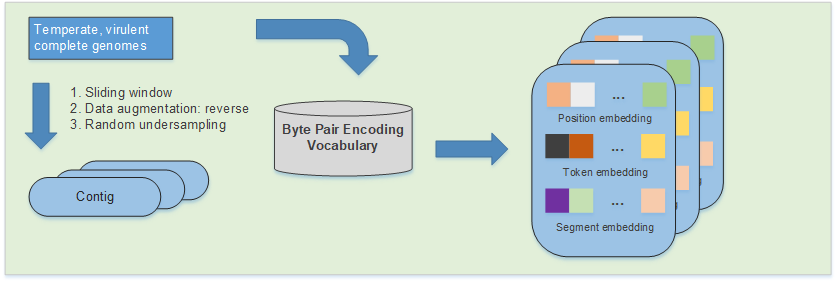
\includegraphics[width=\textwidth]{imgs/data_preparation.png}
%         \caption{Data preparation.}
%         \label{fig:2a}
%     \end{subfigure}
    
%     \vspace{1em}
    
%     \begin{subfigure}{\textwidth}
%         \centering
%         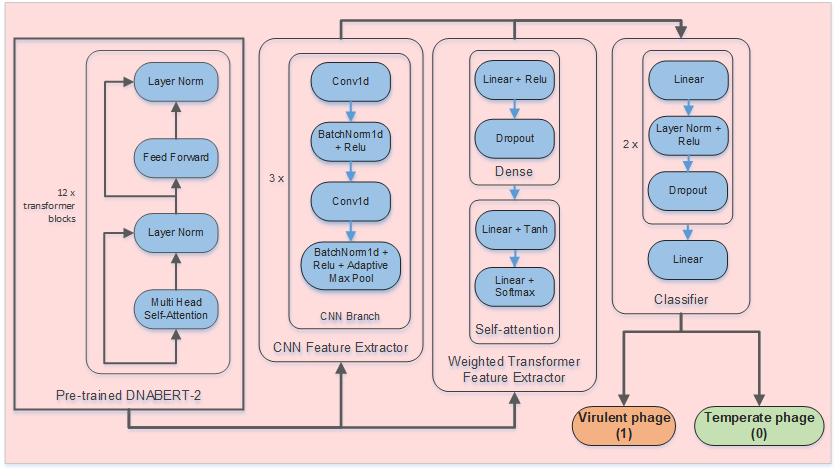
\includegraphics[width=\textwidth]{imgs/model.png}
%         \caption{DNABERT-2 based model.}
%         \label{fig:2b}
%     \end{subfigure}
%     \caption{An overview of DNABERT-2-based pipeline for predicting phage lifestyle.}
%     \label{fig:2}
% \end{figure}

% Both training phases utilize mixed-precision training with automatic mixed precision (AMP) to reduce memory consumption and accelerate computation on GPU hardware. We employ binary cross-entropy loss as the optimization objective for the phage lifestyle classification task. This progressive fine-tuning methodology—initializing task-specific layers before joint optimization—has been demonstrated to improve convergence stability and final performance when adapting pre-trained language models to downstream tasks \cite{howard2018universal, devlin2019bert}, particularly in scenarios where the downstream task involves architectural components not present during pre-training.

\section{Experiments and Results} \label{results}
In this section, we present a comprehensive evaluation of our proposed PhaBERT-CNN model for phage identification across multiple sequence length categories. We conduct (1) a detailed performance comparison between PhaBERT-CNN and DNABERT-2 to demonstrate the effectiveness of domain-specific pre-training combined with convolutional neural networks, and (2) a comparative analysis against state-of-the-art baseline methods, including DNABERT-2, PhaTYP, DeePhage, and ProkBERT, evaluated on four distinct fragment length groups ranging from 100bp to 1800bp. To ensure consistency and fair comparison with previous works, we employ standard binary classification metrics: sensitivity (sn = TP/(TP+FN)), specificity (sp = TN/(TN+FP)), and accuracy (acc = (TP+TN)/(TP+FN+TN+FP)), where sensitivity measures the model's ability to identify virulent phages correctly, specificity assesses accurate detection of temperate phages, and accuracy evaluates overall classification performance. We note that DeepPL was excluded from our benchmark due to the architectural constraints of its underlying DNABERT model, which utilizes learned positional embeddings that impose a maximum input length limitation of 512 bp, rendering it unsuitable for evaluating sequences of up to 1800 bp in our experimental design.

\subsection{PhaBERT-CNN Identification Performance}
\begin{figure}[h]
    \center
    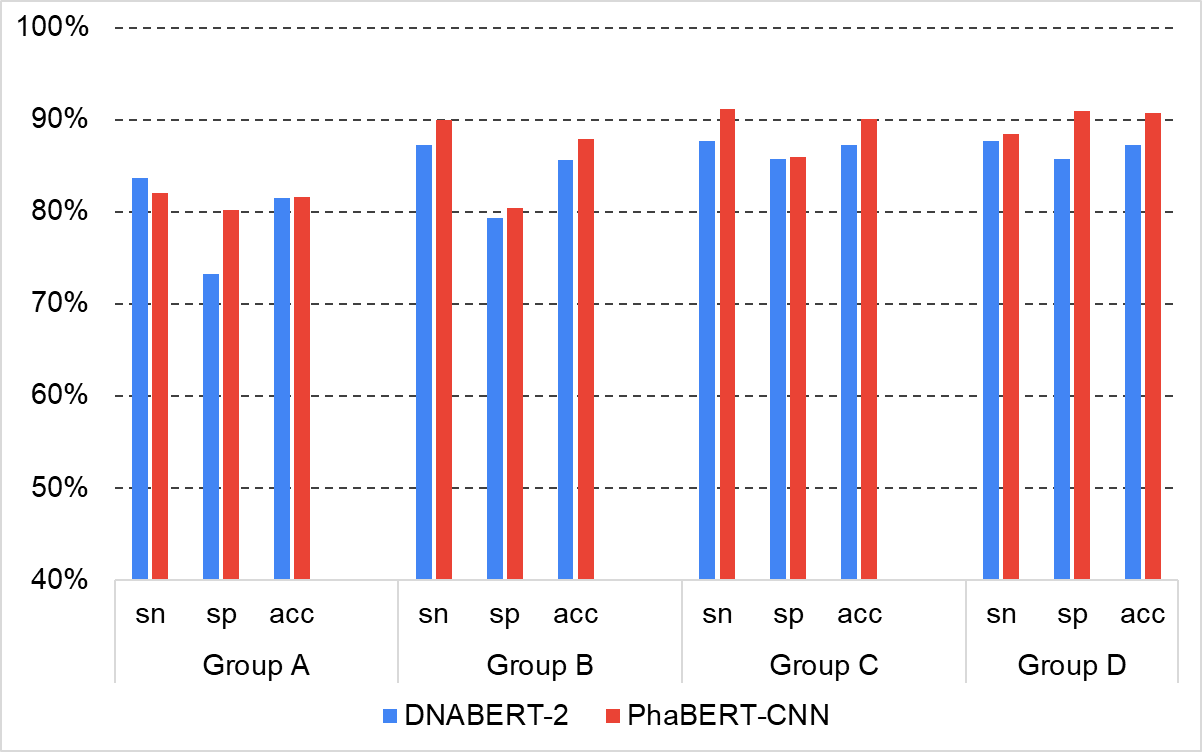
\includegraphics[width=0.8\linewidth]{imgs/dnabert2_vs_phabertcnn.png}
    \caption{Performance comparison of DNABERT-2 and PhaBERT-CNN}
    \label{fig:dnabert2vsphabertcnn}
\end{figure}
To evaluate the performance of our proposed PhaBERT-CNN model against the DNABERT-2 architecture, we conducted a comprehensive comparative analysis across four sequence length groups: Group A (100-400 bp), Group B (400-800 bp), Group C (800-1200 bp), and Group D (1200-1800 bp). The results show in Figure \ref{fig:dnabert2vsphabertcnn} revealed distinct performance patterns that highlight the strengths of our hybrid transformer-CNN approach.

PhaBERT-CNN exhibited superior performance compared to DNABERT-2 consistently across all categories of contig lengths. For Group A, while both models achieved comparable accuracy (DNABERT-2: 81.52\%, PhaBERT-CNN: 81.59\%), PhaBERT-CNN showed substantially improved specificity (80.15\% vs. 73.25\%), representing a 6.90\% gain with minimal sensitivity trade-off. This enhanced specificity is critical for reducing false positives in phage prediction tasks. Performance advantages increased with sequence length: in Groups B and C, PhaBERT-CNN achieved accuracy improvements of 2.35\% and 2.76\%, respectively, with notable sensitivity gains of 2.67\% and 3.44\%. The most pronounced advantage emerged in Group D (1200--1800 bp), where PhaBERT-CNN attained 90.69\% accuracy with balanced sensitivity (88.47\%) and specificity (90.95\%), representing improvements of 3.43\% and 5.20\% over DNABERT-2, respectively. These results suggest that the CNN component effectively captures local sequence patterns and long-range dependencies characteristic of phage genomic signatures, complementing the transformer encoder's global contextual representations.

These results demonstrate that the integration of convolutional layers with transformer-based embeddings in PhaBERT-CNN provides enhanced discriminative capacity for phage identification, particularly for sequences exceeding 400 bp in length, where the model achieves more balanced and robust performance across both sensitivity and specificity metrics.

\subsection{Performance Comparison of Deep Learning-based Methods for Phage Lifestyle Classification}
We conducted systematic strategied 5-fold cross-validation experiments across multiple contig length ranges. Our comparative evaluation encompassed four methods: PhaBERT-CNN, DeePhage \cite{wu2021deephage}, PhaTYP \cite{shang2023phatyp}, and ProkBERT \cite{ligeti2024prokbert}. Following the methodology established by previous studies \cite{wu2021deephage}, we evaluated performance across four contig length groups (A–D), spanning 100–1,800 bp, as described in Section \ref{data_construction}.
\begin{figure}[h]
    \center
    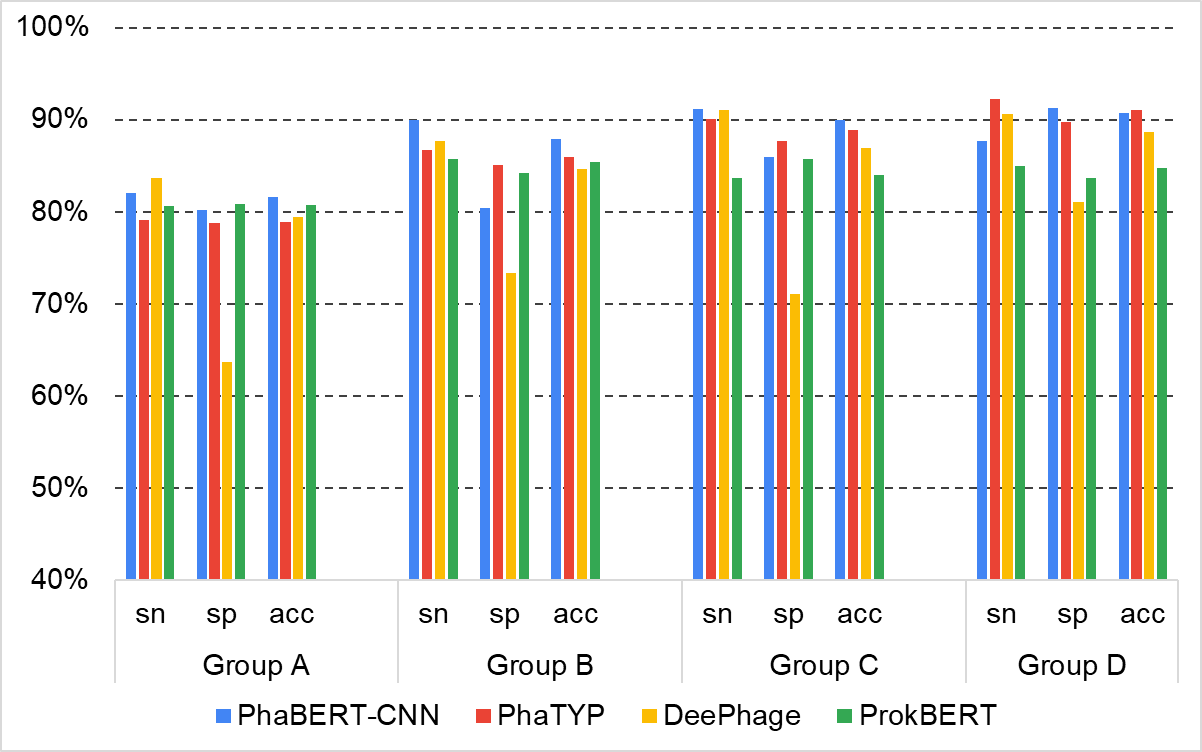
\includegraphics[width=0.8\linewidth]{imgs/primary_contig_exp.png}
    \caption{Identification performance of DeePhage, PhaTYP, and PhaBERT-CNN on group A, B, C, D.}
    \label{fig:exp1}
\end{figure}


\begin{table}[]
\centering
\caption{Performance comparison of PhaBERT-CNN, PhaTYP, DeePhage, and ProkBERT using 5-fold cross-validation on primary contigs.}
\label{tab:1}
\resizebox{\textwidth}{!}{%
\begin{tabular}{rcllll}
\hline
Method &
  Criterion(\%) &
  \multicolumn{1}{c}{\begin{tabular}[c]{@{}c@{}}Group A\\ (100bp - 400bp)\end{tabular}} &
  \multicolumn{1}{c}{\begin{tabular}[c]{@{}c@{}}Group B\\ (400bp - 800bp)\end{tabular}} &
  \multicolumn{1}{c}{\begin{tabular}[c]{@{}c@{}}Group C\\ (800bp - 1200bp)\end{tabular}} &
  \multicolumn{1}{c}{\begin{tabular}[c]{@{}c@{}}Group D\\ (1200bp - 1800bp)\end{tabular}} \\ \hline
\multirow{3}{*}{PhaBERT-CNN} & sn  & 82.00\%                & {\ul \textbf{89.91\%}} & {\ul \textbf{91.12\%}} & 88.47\%                \\
                             & sp  & 80.15\%                & 80.44\%                & 85.93\%                & {\ul \textbf{90.95\%}} \\
                             & acc & {\ul \textbf{81.59\%}} & {\ul \textbf{87.91\%}} & {\ul \textbf{90.01\%}} & 90.69\%                \\ \hline
\multirow{3}{*}{PhaTYP}      & sn  & 79.07\%                & 86.74\%                & 90.09\%                & {\ul \textbf{92.29\%}} \\
                             & sp  & 78.77\%                & {\ul \textbf{85.06\%}} & {\ul \textbf{87.65\%}} & 89.75\%                \\
                             & acc & 78.92\%                & 85.90\%                & 88.87\%                & {\ul \textbf{91.02\%}} \\ \hline
\multirow{3}{*}{DeePhage}    & sn  & {\ul \textbf{80.09\%}} & 86.46\%                & 89.17\%                & 91.17\%                \\
                             & sp  & 71.79\%                & 77.18\%                & 80.13\%                & 80.84\%                \\
                             & acc & 78.07\%                & 84.17\%                & 87.40\%                & 89.09\%                \\ \hline
\multirow{3}{*}{ProkBERT}    & sn  & 80.65\%                & 85.67\%                & 83.61\%                & 85.00\%                \\
                             & sp  & {\ul \textbf{80.80\%}} & 84.15\%                & 85.72\%                & 83.68\%                \\
                             & acc & 80.68\%                & 85.35\%                & 84.03\%                & 84.73\%                \\ \hline
\end{tabular}%
}
\end{table}

Figure \ref{fig:exp1} illustrates the classification performance of the four methods across contig length Groups A, B, C, and D, with detailed results provided in Table \ref{tab:1}. PhaBERT-CNN demonstrated superior and consistent performance across all contig length groups, achieving the highest accuracy of 81.59\% for Group A, 87.91\% for Group B, and 90.01\% for Group C. Notably, PhaBERT-CNN maintained high sensitivity (82.00\%--91.12\%) while achieving competitive specificity (80.15\%--85.93\%) for Groups A through C, indicating balanced performance in identifying both virulent and temperate phages.

PhaTYP exhibited strong performance, particularly on longer contigs\cite{shang2023phatyp}, achieving 92.29\%, 89.75\%, and 91.02\% for sensitivity, specificity, and accuracy, respectively, on Group D. These results suggest that PhaTYP effectively leverages additional sequence information available in longer contigs. However, the method demonstrated lower sensitivity compared to PhaBERT-CNN on shorter contig groups (Groups A, B, C). DeePhage showed moderate performance\cite{wu2021deephage}, with accuracy ranging from 78.07\% to 89.09\% across the four length groups. ProkBERT achieved comparable performance to DeePhage, with accuracy ranging from 80.68\% to 85.35\%. Notably, unlike other methods that exhibited consistent improvement with increasing contig length, ProkBERT demonstrated performance stagnation for longer contigs, with accuracy peaking at 85.35\% in Group B before declining to approximately 84\% in Groups C and D. This pattern suggests potential limitations in ProkBERT's ability to effectively capture long-range dependencies or complex sequence patterns present in extended genomic fragments.

\section{Discussion}\label{discussion}
This study presents PhaBERT-CNN, a hybrid deep learning framework integrating DNABERT-2 transformer embeddings with convolutional neural networks for bacteriophage lifestyle classification from metagenomic contigs. Our evaluation demonstrates competitive performance compared to state-of-the-art methods while addressing critical limitations of existing approaches.

PhaBERT-CNN outperforms the DNABERT-2\cite{zhou2023dnabert} foundation model alone through a hybrid architecture that achieves strong and balanced performance across varied contig lengths. This improvement derives from two complementary components: (1) multi-scale CNN branches (kernel sizes 3, 5, 7) capturing local patterns at different receptive field scales from DNABERT-2 embeddings, and (2) attention-based pooling that computes weighted summation across DNABERT-2 token embeddings to derive a unified sequence representation. The architectural design enables effective multi-scale feature extraction and attention-weighted global aggregation, which become increasingly important for accurate classification of longer genomic sequences. Our model demonstrates superior classification performance for Groups A, B, and C, establishing its effectiveness for fragmented sequences commonly encountered in metagenomic assemblies. For Group D, where PhaTYP exhibits its particular strength, PhaBERT-CNN achieves comparable performance, demonstrating competitive results across the entire spectrum of contig lengths.

PhaBERT-CNN addresses several critical limitations of existing tools. Unlike PhaTYP, which depends on Prodigal\cite{hyatt2010prodigal} for protein detection and fails when proteins are not detected, our approach operates directly on raw DNA sequences, enabling classification even on short contigs lacking complete protein-coding regions—a common scenario in fragmented metagenomic assemblies. Compared to DeePhage's CNN on one-hot encoded sequences, PhaBERT-CNN leverages pre-trained representations capturing complex patterns from diverse genomic data. DNABERT-2 addresses fundamental limitations of earlier models (DNABERT, ProkBERT), including information leakage from overlapping k-mer tokenization and poor computational efficiency.

Despite these advances, several limitations warrant consideration. First, random undersampling for class imbalance may result in information loss. Future work should evaluate alternative resampling strategies or class weighting approaches while maintaining computational feasibility. Data augmentation techniques leveraging DNA's double-strand structure could enhance robustness. Second, while our evaluation demonstrates strong performance on complete genomes and simulated contigs, validation on additional real metagenomic datasets from diverse environments would further establish generalizability.

In conclusion, PhaBERT-CNN advances computational phage lifestyle prediction by effectively combining DNABERT-2 with multi-scale CNN and attention-based pooling architectures. By operating directly on raw DNA sequences and leveraging efficient foundation model representations, PhaBERT-CNN provides a robust solution for metagenomic phage lifestyle classification, establishing a promising paradigm combining pre-trained genomic foundation models with specialized architectures for downstream biological sequence analysis tasks.


\bibliographystyle{splncs04}
\bibliography{references.bib}
\end{document}
